\section{Sprint Maintenance}

Managing Sprints
\newline\newline
With the application if you wish to make a sprint you can create it using similar buttons to other model types. To create a sprint it must have at least a name, an associated backlog, an associated release, a team working on the sprint and a start and end date. Obviously the release must be before or on the end date, and the end date can not be before the start date.

\begin{figure}[H]
\centering
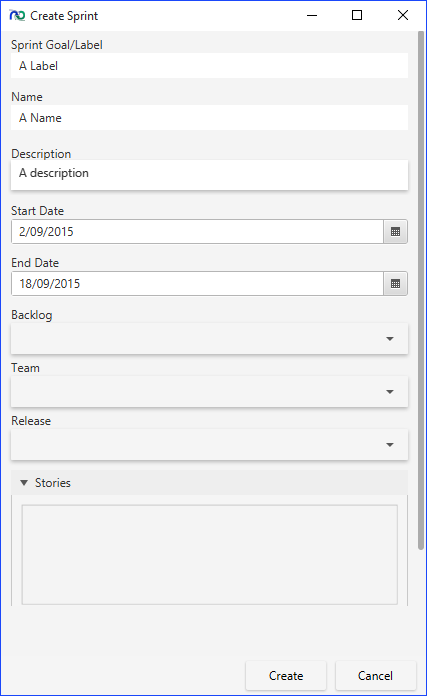
\includegraphics[width=\textwidth]{images/screenshots/sprint1.PNG}
\caption{Creating a Sprint}
\label{fig:new_project}
\end{figure}

You can then add stories to the sprint from the backlog you have assigned it. If you change the backlog you've assigned it too after adding stories it will warn you as it will remove all the stories that you've added to the sprint so far.\newline
\textit{Note: you cannot add a story to multiple sprints.}

From the tabs in the sprint view, the "All Tests" view shows you all the tasks that are in the sprint. These tasks can be filtered by allocated (tests that have people assigned to them) and unallocated (no one is assigned to them). They can also be ordered alphabetically by name, by the story state or their current estimate. Another feature is that you can group them into their corresponding stories, as shown in figure 52.

\begin{figure}[H]
\centering
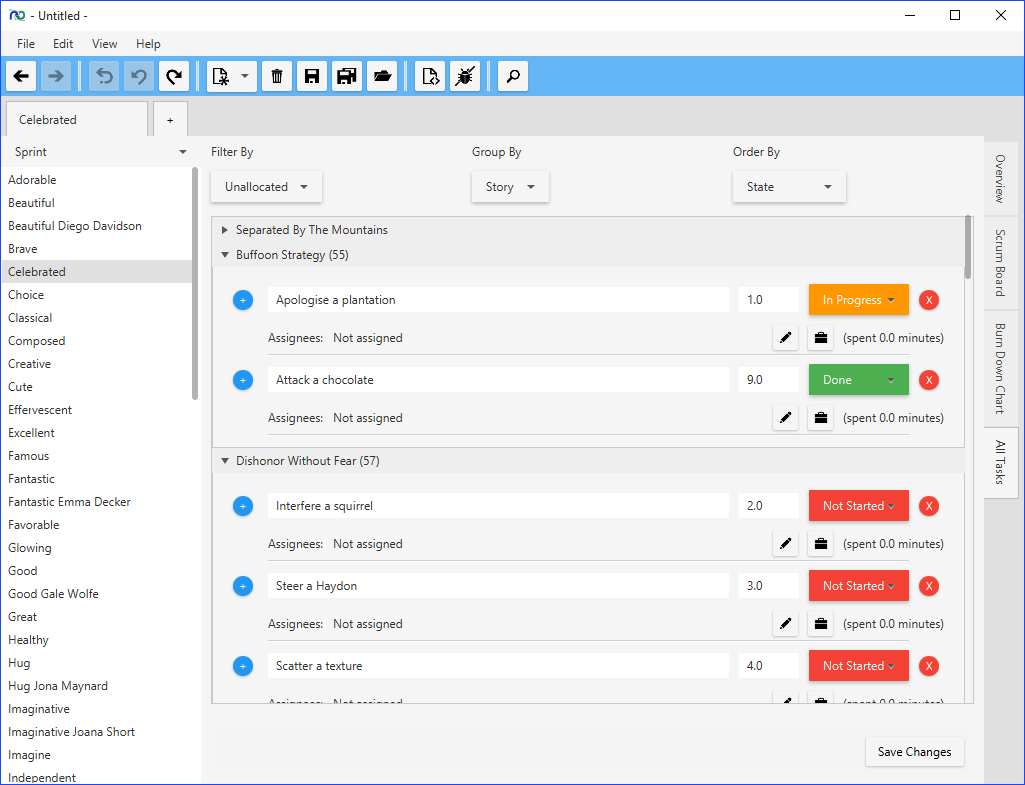
\includegraphics[width=\textwidth]{images/screenshots/sprint2.PNG}
\caption{Viewing all Tasks in a Sprint}
\label{fig:new_project}
\end{figure}

\begin{figure}[H]
\centering
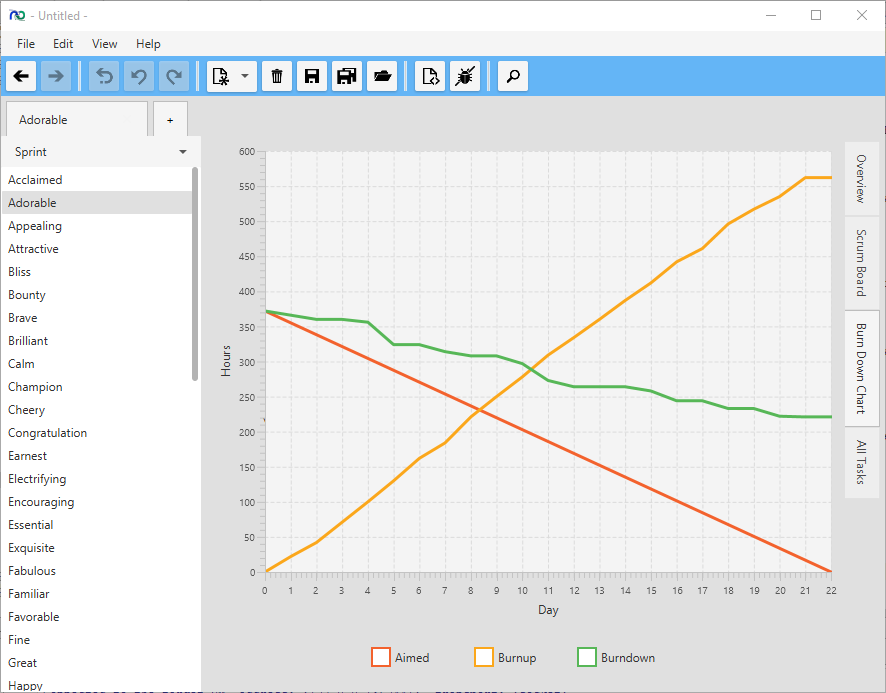
\includegraphics[width=\textwidth]{images/screenshots/burndown.png}
\caption{An example burndown chart}
\label{fig:burndown}
\end{figure}

Switching to the burndown tab will show a burndown graph for the currently selected sprint, as shown in figure 53.

\textbf{Note:}\newline
A graph will only be shown if the sprint has tasks.

Within the sprint editor you can also access a virtual scrum board; figure 54 shows a scrum board. Within this view you can get an overview for all the stories that are within the sprint and the current state of all the tasks within each story. If you want you can expand the story and see all the tasks within it.

Once you are in this view you can drag tasks between the columns (not started, in progress and done). Once all the tasks are in the done column you can mark the story as done.

\begin{figure}[H]
\centering
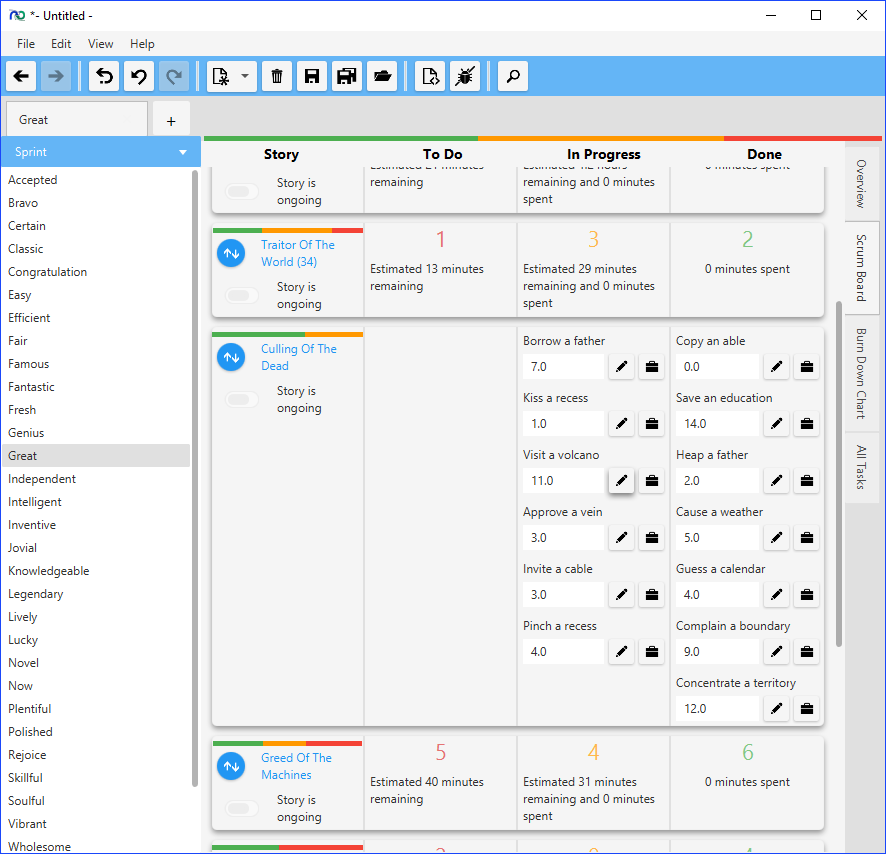
\includegraphics[width=\textwidth]{images/screenshots/scrumboard.png}
\caption{Virtual Scrum Board}
\label{fig:srumboard}
\end{figure}

At the top of this view there is also a bar that indicates the overall completeness of a sprint and all it's contained stories.